\documentclass[11pt,journal]{IEEEtran}
\usepackage{tikz}

\usepackage{times}
\usepackage{amssymb}
\usepackage{amsmath,amsfonts}
\usepackage{amsthm}
\usepackage{graphicx}

\usepackage{color}
\usepackage{xcolor}
\usepackage{pgfgantt}
\usepackage{lscape}
\usepackage{scalefnt}
\usepackage{graphicx}
\usepackage{caption}

\usepackage{pgf}
\usepackage{tikz}
\usetikzlibrary{shapes.symbols,shapes.callouts,snakes,shapes.geometric,arrows}

\usepackage{hhline}
\usepackage{multirow}
\usepackage{array}
\usepackage{pdfpages}
\usepackage{subfigure}
\usepackage{algorithm}
\usepackage[noend]{algpseudocode}
\usepackage{balance}
\usepackage{epsfig}
\usetikzlibrary{shapes,arrows}

\newcommand{\todo}[1]{} %essentially a block comment

\newtheorem{theorem}{Theorem}
\newtheorem{definition}{Definition}
\newtheorem{lemma}{Lemma}

\hyphenation{designs design algo-rithms devel-oped micro-pipeline after
  algo-rithm AFSM AFSMs}

\begin{document}

\title{Volumetric Display}

\author{Semrah Odobasic, Logan Allen, Jin Jeong
  \thanks{The authors are in the Computer Engineering
    department at the University of Utah.}
}
\maketitle

\begin{abstract}
 Volumetric three-dimensional displays are displays which give viewers a sense of depth and immersion by displaying an image in a three-dimensional space. The motivation for such technology is the fact that viewers can be more immersed into the content they are viewing. Specifically they can offer more accurate representations of three-dimensional objects. This method involves taking a light emitting diode matrix and spinning it. As it’s spinning the matrix will be displaying different slices of a three dimensional image. These slices then form a three dimensional volumetric image.


\end{abstract}

\section{Introduction \& Motivation}

\IEEEPARstart{T}{he} project is inspired to push the boundaries of technology and create an immersive experience by designing a volumetric display using a light emitting diode (LED) Matrix. The exciting part comes from merging art with this type of technology. This unique medium allows for a viewer to be more immersed into the content they are viewing and provides multiple unique perspectives for enjoying the same image. This project aims to present three-dimensional (3D) models onto a volumetric display to demonstrate this particular display technology.

The project is driven by a spinning LED matrix which showcases different slices of a 3D model, creating a hologram-like effect \cite{Sun2012ADP}. The project has an LED matrix, high-performance motor, motor driver, IR emitter/receiver, and a microcontroller which drives the motor and matrix. This integrated system is housed on a 3D printed platform, purposefully designed to accommodate each individual hardware component. The motor is attached to the 3D printed platform and is responsible for the rotational movement of the entire system. As everything is attached to the motor and rotates together, there is no need to implement slip rings or other power delivery methods to individual components, simplifying the overall design. The design is small enough that it is able to be held in your hand. This allows it to be visually compelling and easily demonstrable versions of the concept. As part of the demonstration, the project will take a 3D model and present it on the volumetric display.


% Refer to figures as follows:
% The circuit in Fig.~\ref{fig:circuit}.

% Citations are as follows
% Algorithm returning longest netlist delay path \cite{knuth:book1973}.


\section{Background}

In a video online, a small volumetric display was developed and shown by user mitxela on YouTube which uses an LED matrix, WaveShare RP2040 microcontroller, and small CD drive motor to generate 3D images \cite{mitxela_candle}. Additionally, he incorporated an IR sensor on the side of his display which he uses as the primary control method for both motor speed and timing the illumination of the display. By placing a finger in front of the sensor, it then detects the reflected IR light and begins powering the motor and LED matrix. The frequency of the reflected IR light is then used for animation control to display preloaded animations from the RP2040’s flash memory. 

\begin{figure}[h]
    \centering
    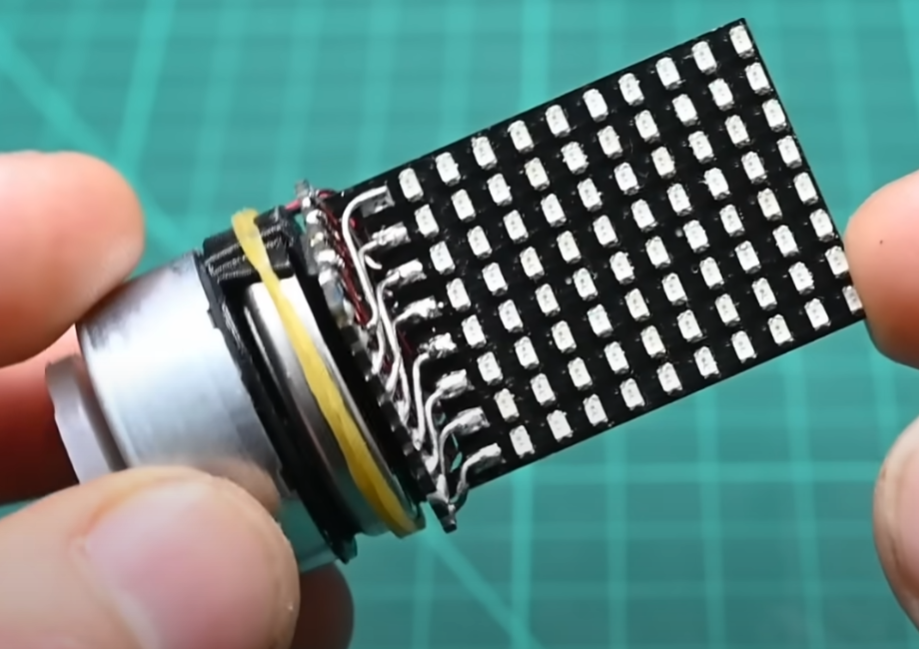
\includegraphics[width=0.5\textwidth]{Mitxela Display.png}
   
    \caption{Mitxela's Volumetric Display.}
    \label{fig: mitxela display}
\end{figure}

While the five minute video primarily displays the final product and its primary design features, mitxela also provides an online project log detailing each step of the design process itself which led him to his final working display. Here, a consideration of the design challenges faced, how those challenges were overcome, and much more detail into the physical and software components utilized to make the final product were made and used as referenced in the creation of this project. 

From mitxela’s online project log itself, there was enough information to not only generate a bill of materials, but to also guide the process of making a similar volumetric display. Even though a great level of insight into his design process was provided, a lot of the information regarding the engineering itself was left out, leaving plenty of decisions to be made in the process of completing the design for this project.

\section{The Design}
The design itself follows the block diagram shown below in Fig. \ref{fig: func diagram} and revolves around the LED matrix as the primary display for producing images. To generate volumetric data, a 3D model or animation will be produced in Blender and split it into slices following the resolution of the display. The design will then use 12 slices of each animation frame so the matrix will need to update itself 12 times for each full rotation of the motor \cite{Sun2014AnID}. These slices are then what creates the volumetric or hologram-like effect desired. The slices generated from Blender and are then converted into binary for use by the microcontroller. 

\begin{figure}[h]
    \centering
    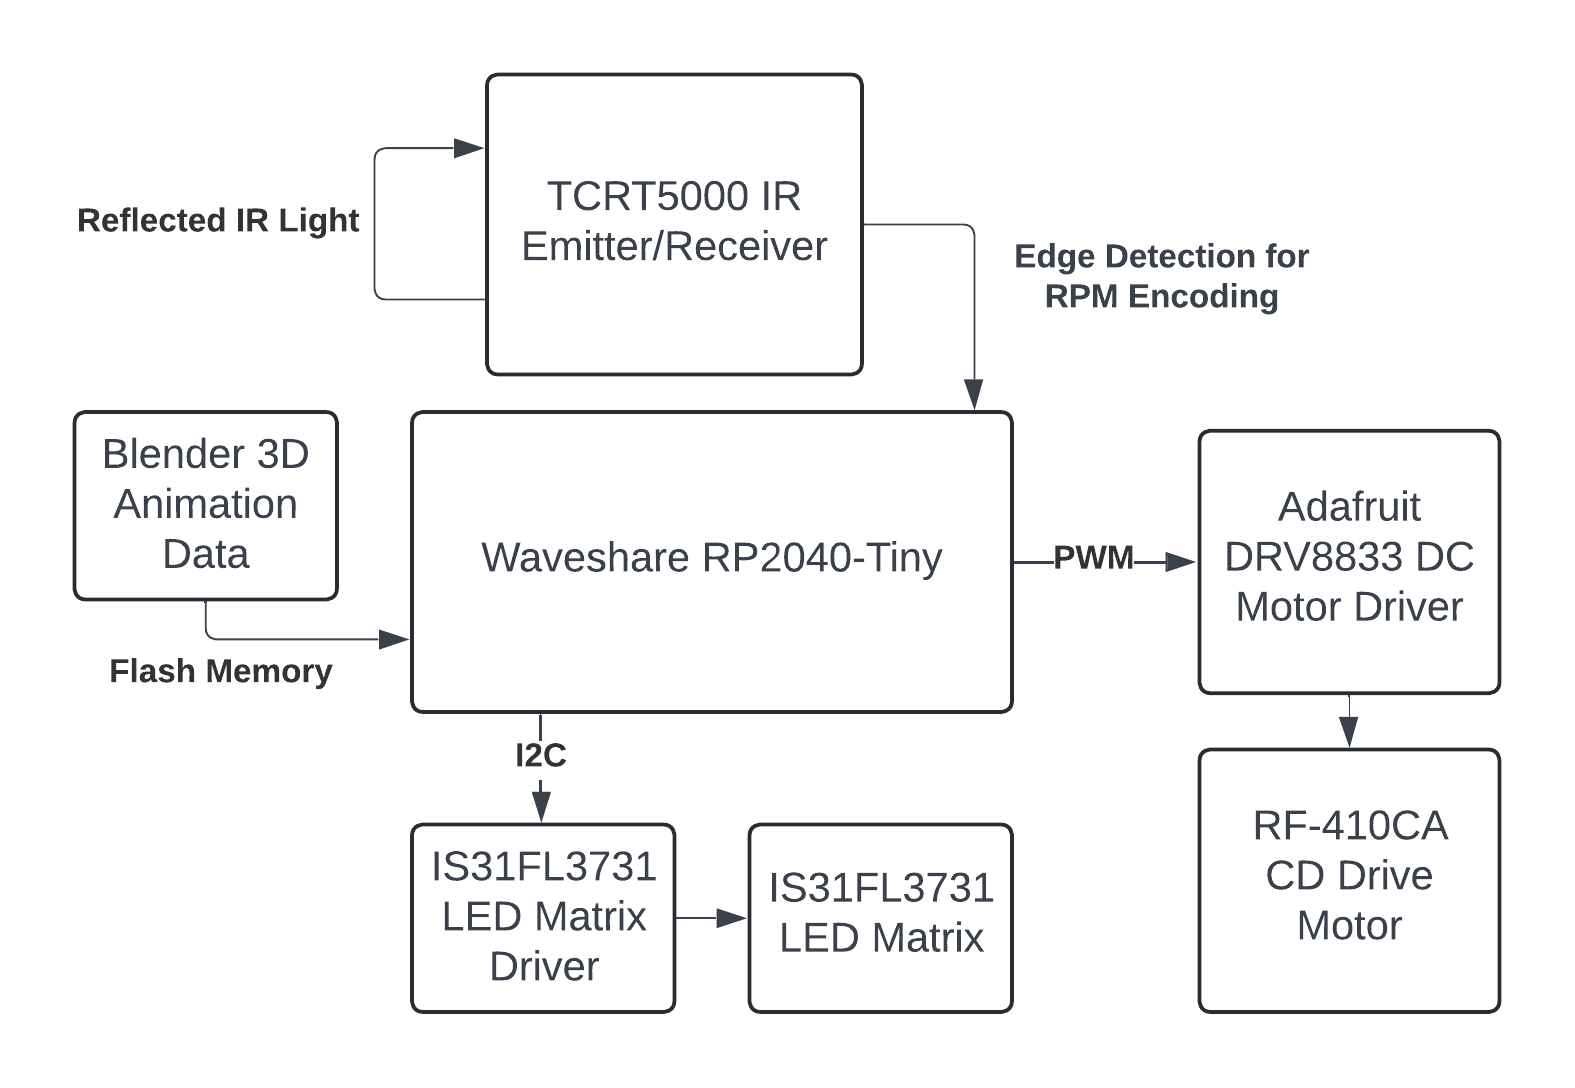
\includegraphics[width=0.5\textwidth]{Block Diagram.png}
   
    \caption{Functional Diagram}
    \label{fig: func diagram}
\end{figure}

The microcontroller itself is also in control of which slice are being displayed at any given moment. It determines this by calculating the RPM that the entire assembly is rotating at via the IR emitter/receiver. By using a reflective surface at a fixed location, the emitter/receiver can track how often it passes that object and translate that into an RPM calculation. Using this RPM reading, the microcontroller will then be capable of displaying frames at the proper interval. The motor is then driven at a fixed speed using pulse width modulation (PWM) that the microcontroller then updates depending on if the assembly is currently rotating too fast or too slow. The motor driver is implemented to ensure that the motor has the power it needs without surpassing any limitations of the microcontroller and provides additional protection against flyback current with the inductive load of the motor.

%% This is a figure with two side by side images.
% \begin{figure}[thb]\centering
%   \begin{minipage}{0.48\columnwidth}
%     \centerline{\psfig{file=images/IMG_2712-crop.jpg, height=30mm, angle=0}}
%     \begin{center} (a) \end{center}
%   \end{minipage}
%   \begin{minipage}{0.5\columnwidth}
%     \centerline{\psfig{file=images/img2.png, height=30mm, angle=0}}
%     \begin{center} (b) \end{center}
%   \end{minipage}
%   \caption{The die and substrate (a), and complete system (b).}
%   \label{fig:chip-system}
% \end{figure}

% This is how you label a section of the text:
% \label{sec:falsePath}

\section{Proposed Work}

The WaveShare RP2040 will be used as the microcontroller due to its small size and large flash capacity cite{3}. It also features two inter-integrated circuit (I2C) busses as well as an analog to digital (ADC) converter. This will allow the RP2040 to drive the display while still having an I2C bus available for any possible stretch goals. An AdaFruit IS31FL3731 LED Matrix will be used as the primary display as it provides a hardware driver that interfaces with the microcontroller and display through I2C to control the LEDs. To spin the display, an RF-410CA CD drive motor will be used due to its size and ability to run at high RPMs. This will ensure that the correct rotational speed is achieved in order to tightly control the switching between animation frames to create a proper 3D image. 

The baseline deliverable will be to have the Waveshare RP2040, AdaFruit LED array \& driver, and RF-410CA displaying a volumetric image. These are the tasks involved for getting a working product:

\begin{enumerate}
    \item Configure tool-chain for programming the RP2040 using C. Demonstrate by controlling the LED on the RP2040.
    \begin{itemize}
        \item Required Resources:
        \begin{itemize}
            \item Linux OS and RP2040.
        \end{itemize}
        \item Estimated Effort:
        \begin{itemize}
            \item Standard debugging for issues that occur with switching languages/IDEs.
        \end{itemize}
    \end{itemize}
    \item Convert AdaFruit IS31FL3731 library used to control the LED matrix driver from Python to C and display an image on the matrix.
    \begin{itemize}
        \item Required Resources:
        \begin{itemize}
            \item MicroPython Library.
        \end{itemize}
        \item Estimated Effort:
        \begin{itemize}
            \item The bulk of the work will come from dissecting the existing Python library and converting it from an interpreted language to a typed language in C. This will take significantly less time and effort however if an existing C library can be found online. 
        \end{itemize}
    \end{itemize}
    \item Control motor using PWM and IR Sensor.
    \begin{itemize}
        \item Required Resources:
        \begin{itemize}
            \item RF-410CA Motor and RP2040.
        \end{itemize}
        \item Estimated Effort:
        \begin{itemize}
            \item Some time will need to be spent learning how the TCRT5000 IR sensor works in order to determine the speed of the motor and rotating display based on the frequency of IR pulses reflected back. Using that, PID control principles will then be utilized to set the speed of the motor to ensure timing is correct for the animation frame rate.
        \end{itemize}
    \end{itemize}
    \item Extract 3D data from Blender
    \begin{itemize}
        \item Required Resources:
        \begin{itemize}
            \item Blender
        \end{itemize}
        \item Estimated Effort:
        \begin{itemize}
            \item Basic 3D models need to be created along with animations. Those 3D models will need to be sliced using a script (likely Python) so that they can be exported to the RP2040 to be displayed.
        \end{itemize}
    \end{itemize}
    \item Display 3D data to LED matrix
    \begin{itemize}
        \item Required Resources:
        \begin{itemize}
            \item RP2040, IS31FL3731 library for the LED matrix and driver, and C program.
        \end{itemize}
        \item Estimated Effort:
        \begin{itemize}
            \item This task will require a C program which takes the blender frames and displays them. This will be done by parsing the display data, displaying that data for a certain time depending on a given RPM, and then repeating when all frames have been parsed. Initially this will be done without spinning to verify data is being displayed correctly.
        \end{itemize}
    \end{itemize}
    \item Combine everything into a volumetric display.
    \begin{itemize}
        \item Required Resources:
        \begin{itemize}
            \item RP2040, IS31FL3731 library, Blender Data, C Program, and RF-410CA.
        \end{itemize}
        \item Estimated Effort:
        \begin{itemize}
            \item All tasks will be combined to create a working model. This model will spin when a hand or object is placed next to the IR sensor. As the model spins it will determine its RPM using the IR sensor. The PWM of the motor will then be set so that the RPM matches a given RPM to ensure the volumetric data is displayed correctly.
        \end{itemize}
    \end{itemize}
\end{enumerate}



\subsection{Required Components}

Following the table of bill of materials, this is our required components:

For the initial stage, custom PCBs will not be required. This may change depending on future stretch goals that will be determined later in the project. All of the current components are subject to change depending on how the project develops.

\begin{table}[h]
\centering
\caption{Bill of Materials (BOM)}
\begin{tabular}{|p{3cm}|p{5cm}|}
\hline
\textbf{Component} & \textbf{Description} \\
\hline
Waveshare RP2040 Tiny Micro-controller & Micro-controller used to drive the entire assembly. \\
\hline
AdaFruit Charlieplexed LED Array & 9x16 LED array using blue LEDs. \\
\hline
AdaFruit LED Array Driver & Recommended part to simplify interfacing with the LED array. \\
\hline
RF-410CA Motor & Small CD motor for rotating the display. \\
\hline
TCRT5000 IR Sensor & IR emitter and receiver used to encode motor speed. \\
\hline
LIR2450 Battery & Rechargeable battery to power the assembly. \\
\hline
Flyback Diode & Schottky diode soldered with the motor control to prevent reverse current. \\
\hline
SOT-23 Mosfet & Wired with the motor control circuit. \\
\hline
3D Printed Battery Holder & Custom 3D printed holder for the battery and other components. \\
\hline
Solid Core and Enamel Wire & Wiring for electrical components. \\
\hline
\end{tabular}

\end{table}

\subsection{Task Interfaces}

Fig. \ref{fig: func diagram} demonstrates how every component interfaces with different peripherals. The individual components are all connected via different interfaces with the RP2040 Tiny being the center. The LED matrix is connected to the microcontroller via an I2C connection and is interfaced using a custom C library which follows the provided Adafruit library in C++ and Micropython. The motor is driven by PWM through a motor controller. The reason for this is to isolate the power the motor uses to ensure no limits are being passed on the microcontroller. The IR transmitter/receiver is a simple module. One half is an IR emitting diode which is simply connected to power and ground with a resistor. The other half is the receiving section which is a phototransistor. This is also connected to power via a resistor with the voltage across the phototransistor being measured by the GPIO. This GPIO is how the microcontroller measures RPM, it detects the amount of time between falling edges. All of this is attached onto the 3D print which holds the parts together cleanly.

\subsection{Testing and Integration Strategy}
During the prototyping stage, each component of the project will be done in individual testing to ensure functionality. This approach guarantees that elements such as the Waveshare RP2040 micro-controller, LED matrix, and motor are operating correctly independently. The testing process involves establishing proper hardware connections through soldering, verifying the micro-controller functionalities with C programming, and assessing the LED array's responsiveness to control signals using Arduino  example code and existing libraries. This ''incremental testing'' method will be essential for identifying and resolving any initial issues encountered.

Once each component is confirmed to be operational, the project will progress to system integration testing. This phase will involve combining all elements with  soldering  to ensure stability and connectivity. With a solid hardware setup, the testing focus will shift to evaluating the good usage between the micro-controller and its peripherals. This testing phase will ensure that the overall functionality of the volumetric display with all components connected and working together.

Specifically, testing will include examining the LED matrix at varying frame rates, observing the motor's response to control signals, and validating the synchronization between the LED matrix, motor, and IR sensor. Efforts will also be dedicated to debugging and resolving any hardware-software integration challenges. This ensures that the LED matrix displays the correct slices of the 3D model at the appropriate moments during rotation.

The ''System integration testing'' phase will address any bugs encountered when different components interact, providing flexibility to incorporate new components in the future. Through this comprehensive and integrated testing process, our team aims to systematically validate each component as it's assembled into the final product.


\subsection{Schedules and Milestones}


\begin{table}[h]
\centering
\caption{Milestone Schedule}
\begin{tabular}{|c|p{3cm}|p{3cm}|}
\hline
\textbf{Milestone} & \textbf{Description} & \textbf{Target Date} \\
\hline
1 & Configure tool-chain for RP2040 programming in C & April 19 \\
\hline
2 & Convert AdaFruit IS31FL3731 library to C and display image on LED matrix & Aug. 9 \\
\hline
3 & Implement motor control using PWM and IR Sensor & August 23 \\
\hline
4 & Extract 3D data from Blender & Sept. 13 \\
\hline
5 & Display 3D data on LED matrix & Oct. 4 \\
\hline
6 & Integrate all components into a volumetric display & Nov. 1 \\
\hline
7 & Stretch goal: Scale and improve prototype & December 6 \\
\hline
\end{tabular}
\end{table}

\subsection*{1. Configure tool-chain for RP2040 programming in C}
\begin{itemize}
  \item \textbf{Time Estimation:} 2 weeks
\end{itemize}

\subsection*{2. Convert AdaFruit IS31FL3731 library to C}
\begin{itemize}
  \item \textbf{Time Estimation:} 4-6 weeks
  \item \textbf{Additional Details:} 
  \begin{itemize}
    \item This milestone may take a lot of time, so additional time is allotted.
  \end{itemize}
\end{itemize}

\subsection*{3. Implement motor control using PWM and IR Sensor}
\begin{itemize}
  \item \textbf{Time Estimation:} 2 Weeks
  \item \textbf{Additional Details:} 
  \begin{itemize}
    \item Timing protocols can be tricky but prior experience will significantly reduce potential complications.
  \end{itemize}
\end{itemize}

\subsection*{4. Extract 3D data from Blender}
\begin{itemize}
  \item \textbf{Time Estimation:} 3 Weeks
\end{itemize}

\subsection*{5. Display 3D data on LED matrix}
\begin{itemize}
  \item \textbf{Time Estimation:} 3 Weeks
  \item \textbf{Additional Details:} 
  \begin{itemize}
    \item Timing the animations based on rotation speed of the matrix.
    \item Plan to pre-process animations from Blender.
  \end{itemize}
\end{itemize}

\subsection*{6. Integrate all components into a volumetric display}
\begin{itemize}
  \item \textbf{Time Estimation:} 1 Month
  \item \textbf{Additional Details:} 
  \begin{itemize}
    \item Integration can also produce complications, but mitxela provides reference code and a project log documenting his implementation of the project. This will be referenced as needed for debugging or further idea generation.
    \item Prototyping and breadboarding each sub-circuit before final assembly.
  \end{itemize}
\end{itemize}

\subsection*{7. Stretch Goal: Scale and improve the initial prototype}
\begin{itemize}
  \item \textbf{Time Estimation:} 1 Month
  \item \textbf{Additional Details:} 
  \begin{itemize}
    \item Utilize remaining time to enhance the prototype.
    \item Adjust schedule if needed based on progress of initial milestones.
  \end{itemize}
\end{itemize}


\subsection{Preliminary Risk Assessment}



Converting the AdaFruit IS31FL3731 Library from Python to C poses a high risk due to inexperience with code conversion between these two languages. To mitigate this risk, the communication process itself may need to be reverse engineered using a basic knowledge of I2C in order to reconstruct the library’s basic functions in C. In rewriting this library, custom abstractions will also be utilized such that the library itself interfaces smoothly with the rest of the project and is easy to read. The target date for reducing this risk from red to yellow is set for the end of Spring semester.

The task of extracting 3D data from Blender involves running C\# scripts over the software, a process which is relatively new to the team and presents a yellow risk level. To mitigate this risk, mitxela’s project repository will be referenced in regards to his C\# script, and other resources online will be utilized to troubleshoot any issues that may arise. The target date for reducing this risk to green will be within the first two months of starting the official work on developing the project.



Displaying 3D data on the LED matrix involves timing based on the matrix rotation speed which presents a yellow risk level. To mitigate this risk, the goal will be to to pre-process all animations from Blender into 2D arrays representing which LEDs should turn on when. The software on the RP-2040 tiny will then cycle through each 2D array based on the timing generated by the rotating LED array. Mitxela’s existing codebase will be utilized again for guidance and troubleshooting as needed throughout the development of this software. The target date for reducing this risk to green is set for the end of the Spring semester.

Integrating all hardware peripherals and individual components into a final working volumetric display has potential to introduce new bugs which presents an additional medium risk. To mitigate this risk, each subassembly and individual component will be prototyped on a breadboard before final assembly to ensure components work properly and have well defined interfaces. A block diagram will then be followed to ensure correct integration of all hardware components into the final design. The target date for reducing this risk to green is also set for the end of the Spring semester.

\subsection{Group Management and Communication}

From working together in groups prior to this project, our team has a well structured process already in place for both communication and scheduling time to work on project milestones. In particular, we utilize a private Discord server with channels designated for each project in progress between different classes we collaborate in. This constitutes our physical method of communication to schedule times to meet, document our progress, and hold each other accountable for any individual tasks that may have been assigned.

From working on multiple projects together in the past, our tendency typically relies on group work either in person in a lab on campus, or over video calls through Discord so we each contribute our individual strengths to all steps of the engineering process and keep up to date on progress for each milestone. Luckily, due to being in many similar classes together, our schedules line up rather effortlessly giving us the flexibility to meet at any time throughout the day or week. Additionally, due to our utilization of Discord, we’ve found that we’ve been able to continue working in groups more flexibly even if someone is out of town, or if we need to meet later in the day while we’re all home. Overall, this style of work and communication has allowed us to work quite efficiently in the past, and our plan will be to continue in this format for completing our volumetric display.

Also from following this structure, we don’t typically have to prescribe to traditional methods of reporting on individual tasks, since the majority are completed with all members present. While typically some time could be saved by completing individual tasks in tandem, we’ve found that working as a trio requires less time providing updates in additional meetings or through text to keep each other up to speed on individual work completed. From this collaborative style of work, our team also typically refrains from defining any particular roles such as ''team lead'' given that we all work equally to meet on a consistent basis to make progress on all aspects of the project together. Instead, one team member typically takes the lead on a task such as programming or hardware assembly when we meet, while the rest of the team follows and provides insight or corrections. While in-person collaboration is rather straightforward, we do also utilize screen sharing or live video feeds when working remotely to further facilitate our group work regardless of the task being accomplished.

While the majority of our communication is verbal when we meet to work on projects, we will however use Discord and other task management systems to track progress on our project as a whole throughout development. In following the project design from mitxela, our plan is to use Trello to segment out the individual tasks for completing the volumetric display similar to the steps taken by mitxela to implement his own design. In using Trello, we can then assign tasks to team members based on individual strengths and who will take the lead during group work sessions, and we can further track each task in stages of development to ensure that we’re meeting the timelines set for our milestones. We’ll also use GitHub and Google Drive for document sharing and source control, and Discord for any other forms of communication as described earlier.


 
\section{Conclusion}
Following the design for a mini volumetric display presented by user mitxela on YouTube, this project aims to replicate his model for a swept-volume handheld display. An RP2040-tiny microcontroller provides the primary processing and control for the assembly, while a CD Drive motor rotates an LED array utilizing rotational encoding provided by an infrared receiver/emitter. Once the appropriate rotational speed is achieved, pre-processed animation frames from Blender can then be cycled to create visually appealing, 3D images and animations in the palm of your hand.

While traditional volumetric displays can be quite bulky, complex, and expensive, this design works to be as minimal as possible, while still being convenient to engineer and assemble. In particular, all components of the display rotate together, reducing the need to use slip rings or bearings to provide complicated power delivery to rotating parts. Additionally, with its tactile and compact design, this volumetric display can be directly handled by the user in a way that’s intuitive and engaging, providing an opportunity to explore the relatively nuanced world of truly three-dimensional displays. And overall, while volumetric displays are still in their infancy, this project hopes to provide additional insight into the viability of volumetric displays, providing a clear and simplified framework for producing 3D images for use in new industries and additional niche applications.



\section*{Acknowledgments}

  Donggi Lee, who contributed all the 3D printing for this project. His assistance in both the design and printing of the battery holder and base for the final design significantly contributed to the success of the project.


\bibliographystyle{plain}  % IEEEtran -- needs IEEEtran.bst
% Balance the citations to equalize the columns manually
% \balance
\bibliography{proposal}
\end{document}

% LocalWords:  Eqn df
